\section{Hilbert spaces}

\begin{definition}\label{ii.1}
    Assume that $V$ is a real vector space. A \bol{scalar product}\index{scalar product} is a function $\scalvvr$ with the properties
    \begin{enumerate}[label=\alph*)]
        \item Bilinearity: $\forall y\in V:\, V\ni x\mapsto\scal{x}{y}$ and $\forall x\in V:\,V\ni y\mapsto\scal{x}{y}$ are linear.\label{ii.1.a}
        \item Symmetry: $\forall x,y\in V:\,\scal{x}{y}=\scal{y}{x}$.\label{ii.1.b}
        \item Positivity: $\forall x\in V,x\neq0:\,\scal{x}{x}>0$.\label{ii.1.c}
    \end{enumerate}
\end{definition}

\begin{definition}\label{ii.2}
    If $V$ is a complex vector space \emph{(}i.e. w.r.t. the field $\C$ of complex numbers\emph{)} then $\scalvvc$ with property \ref{ii.1.c} above, but properties \ref{ii.1.a} and \ref{ii.1.b} are changed to
    \begin{enumerate}[label=\alph*)]
        \item Sesquilinearity: $\forall x\in V:\, V\ni y\mapsto\scal{x}{y}$ is linear and $\forall y\in V:\, V\ni x\mapsto \scal{x}{y}$ is \rec{\bol{skewlinear}} \emph{(}or conjugate linear\emph{)}, that is
        \[\scal{x}{\alpha y_1+\beta y_2}=\alpha\scal{x}{y_1}+\beta\scal{x}{y_2}\]
        and
        \[\scal{\alpha x_1+\beta x_2}{y}=\conj{\alpha}\scal{x_1}{y}+\conj{\beta}\scal{x_2}{y}\]
        for all $x,y\in V,\;\alpha,\beta\in\C$.
        
        \item Skew symmetry: $\scal{x}{y}=\conj{\scal{y}{x}}$ for all $x,y\in V$.
    \end{enumerate}
    is also a scalar product.
\end{definition}

\begin{thm}[Cauchy-Schwarz]\label{ii.3}\index{Cauchy-Schwarz}
    A scalar product satisfying \ref{ii.1.a},\ref{ii.1.b} and \ref{ii.1.c} above satisfies
    \[|\scal{x}{y}|\leq\|x\|\|y\|\;\forall x,y\in V\tag{2.1}\label{2.1},\]
    where $\|x\|:=\sqrt{\scal{x}{x}}$. Moreover, equality in \eqref{2.1} holds iff $x=\alpha y$ for some $\alpha\in\R$ \emph{(}or $\C$\emph{)}. i.e., $x$ and $y$ are linearly dependent.
\end{thm}

\begin{cor}\label{ii.4}
    If $V$ is a vector space with a scalar product, then
    \[\|x\|:=\sqrt{\scal{x}{x}}\label{2.3}\tag{2.3}\]
    defines a norm on $V$.
\end{cor}

\begin{cor}\label{ii.5}
    If $V$ is a vector space with a scalar product $\scal{\cdot}{\cdot}$, then
    \[\|x\|=\sup_{\substack{y\in V\\\|y\|=1}}|\scal{y}{x}|.\tag{2.4}\label{2.4}\]
\end{cor}

\begin{prop}[Parallelogram identity]\label{ii.6}\index{parallelogram identity}
    If $V$ is a real vector space with a scalar product, then
    \[\|x+y\|^2+\|x-y\|^2=2\|x\|^2+2\|y\|^2\;\;\;\,\forall x,y\in V\tag{2.5}\label{2.5}\]
\end{prop}

\begin{figure}[!h]
    \centering
    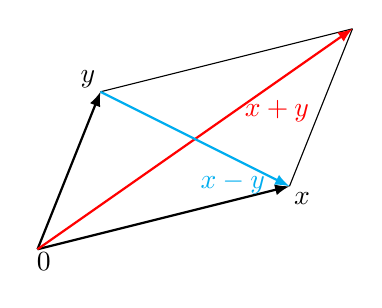
\begin{tikzpicture}[scale=0.8]
        \draw[thick,-{latex[scale=3.0]}] (0,0) -- (4,1);
        \draw[thick,-{latex[scale=3.0]}] (0,0) -- (1,2.5);
        \draw (4,1) -- (5,3.5);
        \draw (1,2.5) -- (5,3.5);
        \node at (4.2,0.8){$x$};
        \node at(0.8,2.7){$y$};
        \draw[red,thick,-{latex[scale=3.0]}] (0,0) -- (5,3.5);
        \draw[cyan,thick,{latex[scale=3.0]}-] (4,1) -- (1,2.5);
        \node[text=red] at (3.8,2.2){$x+y$};
        \node[text=cyan] at (3.1,1.05){$x-y$};
        \node at (0.1,-0.2){$0$};
    \end{tikzpicture}
\end{figure}

\subsection{Convex subsets, Projection Theorem}

Recall that a subset $A\subset V$ is \rec{\bol{convex}}\index{convex} if
\[\forall x,y\in A,\theta\in[0,1]\te{ one has }\theta x+(1-\theta)y\in A.\]
\begin{figure}[!h]\vspace{-5mm}
    \centering
    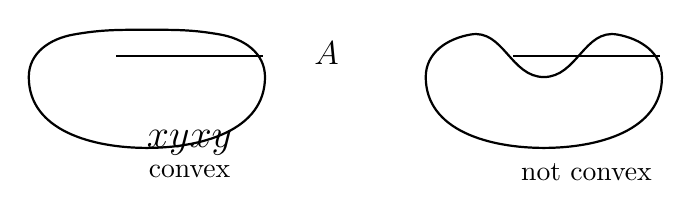
\begin{tikzpicture}[scale=0.3]
    \draw[thick] (0,0) to [out=0,in=270] (5,3) to [out=90,in=350] (3.1,4.8) to [out=170,in=0] (0,5) to [out=180,in=10] (-3.1,4.8) to [out=190,in=90] (-5,3) to [out=270,in=180] (0,0);
    \tdot{-3.1}{3.9}{\Large $x$}{below};
    \tdot{3.1}{3.9}{\Large $y$}{below};
    \draw[thick] (-3.1,3.9) -- (3.1,3.9);
    \node at (5.8,4) {\large $A$};
    \node at (0,-1) {convex};
    
    
    \draw[thick] (0+15,0) to [out=0,in=270] (5+15,3) to [out=90,in=350] (3.1+15,4.8) to [out=170,in=0] (0+15,3) to [out=180,in=10] (-3.1+15,4.8) to [out=190,in=90] (-5+15,3) to [out=270,in=180] (0+15,0);
    \tdot{-3.1+15}{3.9}{\Large $x$}{below};
    \tdot{3.1+15}{3.9}{\Large $y$}{below};
    \draw[thick] (-3.1+15,3.9) -- (3.1+15,3.9);
    \node at (5.8+15,4) {\large $A$};
    \node at (15,-1) {not convex};
    \end{tikzpicture}
\end{figure}

The \bol{\rec{convex hull}}\index{convex!hull} of $A\subset V$ is defined to be
\[\conv(A):=\bigg\{\hspace{-8mm}\underbrace{\sum_{j=1}^ka_jx_j}_{\scriptsize\te{convex linear combination}}\hspace{-8mm}\colon k\in\N,\ x_1,\ldots,x_k\in A,\ a_j\geq0,\ \sum_{j=1}^ka_j=1\bigg\}.\]

Note that $A$ is convex $\Lolrarr\conv(A)=A$. If $A\subset V$ is convex, then a function 
$\func{f}{A}{\R\cup\{\infty\}}$ is \bol{\rec{convex}} if 
\[f(\theta x+(1-\theta)y)\leq\theta f(x)+(1-\theta)f(y)\;\;\;\forall x,y\in A,0\leq\theta\leq 1.\tag{2.6}\label{2.6}\]

A function $\func{f}{A}{\R\cup\{-\infty\}}$ is \bol{\rec{concave}} if $-f$ is convex. 
If $\func{f}{V}{\R\cup\{\infty\}}$ is convex, then the set $\{x\in V\colon f(x)\in\R\}$ is convex 
in $V$ and $B=\{(x,\alpha)\in V\times\R\colon \alpha\geq f(x)\}$ is convex in $V\times\R$.

\begin{thm}[Projection theorem]\label{ii.7}\index{Projection theorem}
    Let $\H$ be a Hilbert space and $A\subset\H$ not empty, closed and convex subset. 
    Then there exists exactly one map
    \[\func{P}{\H}{A}\te{ such that }\|x-P(x)\|=\dist(x,A)=\inf_{y\in A}\|x-y\|.\tag{2.7}\label{2.7}\]
    Moreover, for each $x\in\H$, the point $P(x)\in A$ is characterized by
    \[\mathrm{Re}\scal{y-P(x)}{x-P(x)}\leq0\;\;\forall y\in A.\tag{2.8}\label{2.8}\]

    One calls $\func{P}{\H}{A}$ the \rec{\bol{nearest point projection}}, or the \rec{\bol{orthogonal projection}} from $\H$ to $A$.
\end{thm}

\paragraph{Remarks}
\begin{enumerate}
    \item If $A\subset\H$ is a non-empty, closed \rec{\bol{affine subset}}, that is
    \[x,y\in A,\alpha\in\K\Lorarr(1-\alpha)x+\alpha y\in A\]
    then $\PHA$ is \rec{\bol{affine}}, that is
    \[P((1-\alpha)x_1+\alpha x_2)=(1-\alpha)P(x_1)+\alpha P(x_2)\;\;\;\forall x_1,x_2\in\H,\alpha\in\K.\]
    Moreover, for any $y_0\in A$ and $x\in\H$ the image $P(x)$ is characterized by ("orthonogality" condition)
    \[\scal{y-y_0}{x-P(x)}=0\;\;\;\forall y\in A.\tag{2.8b}\label{2.8b}\]
    
    \item Is $A\subset\H$ a non-empty \bol{\rec{closed subspace}}, i.e.,
    \[y_1,y_2\in A,\alpha,\beta\in\K\Lorarr \alpha y_1+\beta y_2\in A\]
    then the map $\PHA$ is linear and $P(x)\in A$ is characterized by
    \[x-P(x)\perp A\;\te{ i.e., }\scal{y}{x-P(x)}=0\;\;\;\forall y\in A.\tag{2.8c}\label{2.8c}\]
\end{enumerate}

\subsection{A reminder on linear maps between normed vector spaces}

If $X,Y$ are complex vector spaces, then $\TXY$ is \rec{\bol{conjugate linear}} if
\[T(\alpha x_1+\beta x_2)=\conj{\alpha}T(x_1)+\conj{\beta}T(x_2)\;\;\;\forall x_1,x_2\in X,\alpha,\beta\in\C.\tag{2.15}\label{2.15}\]
If $X$ and $Y$ are normed vector spaces with norms $\|\cdot\|_X$ and $\|\cdot\|_Y$, then a function $\TXY$ (linear or not) is continuous at $x_0\in X$ if
\[\forall\varepsilon>0\,\exists \delta>0\,\forall x\in X\te{ with }\|x-x_0\|_X<\delta\colon\,\|T(x)-T(x_0)\|_Y<\varepsilon.\tag{2.16}\label{2.16}\]
$T$ is continuous on $X$ if it is continuous at any point $x_0\in X$ and $T$ is uniformly continuous on $X$ if
\[\forall\varepsilon>0\,\exists\delta>0\,\forall x_1,x_2\in X\te{ with }\|x_1-x_2\|_X<\delta\colon\,\|T(x_1)-T(x_2)\|_Y<\varepsilon.\tag{2.17}\label{2.17}\]

\begin{thm}\label{ii.8}
    Let $(X,\|\cdot\|_X)$, $(Y,\|\cdot\|_Y)$ be normed vector spaces and $\TXY$ linear. Then the following are equivalent
    \begin{enumerate}[label=\alph*)]
        \item $T$ is uniformly continuous.\label{ii.8.1}
        \item $T$ is continuous.\label{ii.8.2}
        \item $T$ is continuous at zero.\label{ii.8.3}
        \item $\|T\|=\|T\|_{X\rarr Y}:=\sup\limits_{\substack{x\in X\\x\neq0}}\frac{\|Tx\|_Y}{\|x\|_X}<\infty$.\label{ii.8.4}
    \end{enumerate}
\end{thm}

\paragraph{Remarks}
\begin{enumerate}
    \item The space $L(X,Y):=\{\TXY\te{ linear and continuous}\}$ is a vector space and $\|\cdot\|_{X\rarr Y}$ is a norm on it.
    \item If $Y$ is a Banach space (i.e., complete) then $L(X,Y)$ with norm $\|\cdot\|_{X\rarr Y}$ is also a Banach space.
\end{enumerate}

\subsection{Continuous linear functionals on Hilbert spaces, Riesz lemma}
Let $\H$ be a Hilbert space. The vector space
\[\H^*:=L(\H,\K)\tag{2.20}\label{2.20}\index{dual space}\]
is called the (vector)space of \rec{\bol{continuous linear functionals}} on $\H$. It has norm
\[\|\ell\|_{\H^*}:=\sup_{x\in\H}\frac{|\ell(x)|}{\|x\|}\tag{2.21}\label{2.21}\]
and
\[\|\ell\|_{\H^*}=\|\ell\|_{\H\rarr\K}=\sup_{\|x\|=1}|\ell(x)|.\]

\begin{lem}[Key lemma]\label{ii.9}\index{Key lemma}\ 
    \begin{enumerate}[label=\arabic*)]
        \item Let $\ell\in\H^*$. Then the \bol{\rec{null space}}\label{ii.9.1}
        $N(\ell):=\{x\in\H\colon\ell(x)=0\}$
        is a closed subspace of $\H$.
        \item Let $\func{\ell_1,\ell_2}{\H}{\K}$ be linear, \rec{(}not necessarily bounded\rec{)} with $N(\ell_1)=N(\ell_2)$ and $\ell_2\neq0$. Then there exists a $\gamma\in\K$ such that $\ell_1=\gamma\ell_2$.\label{ii.9.2}
    \end{enumerate}
\end{lem}

\begin{thm}[Riesz representation theorem, Riesz lemma]\label{ii.10}\index{Riesz representation theorem}
    If $\H$ is a Hilbert space with scalar product $\scal{\cdot}{\cdot}$ then for each $\ell\in\H^*$ there exists a unique $v_\ell\in\H$ such that $\ell=\scal{v_\ell}{\cdot}$, i.e., $\ell(x)=\scal{v_\ell}{x}$ for all $x\in \H$. In other words, the conjugate linear isometric map
    \[\func{J}{\H}{\H^*},\;\;v\mapsto J(v)=\scal{v}{\cdot}\]
    is bijective \emph{(}hence an isomorphism\emph{)}.
\end{thm}

\subsection{Extension of Riesz-Lemma: Lax-Milgram}
\begin{thm}[Lax-Milgram]\label{ii.11}\index{Lax-Milgram}
    Let $\H$ be a Hilbert space over the field $\K$ \emph{(}$=\R$ or $\C$\emph{)} and $\func{a}{\H\times\H}{\K}$ sesquilinear. Furthermore, assume that there are constants $c_0,C_0$ with $0<c_0\leq C_0<\infty$ such that for all $z,x\in\H$
    \begin{enumerate}[label=\arabic*)]
        \item $|a(x,z)|\leq C_0\|x\|\|z\|\label{ii.11.1}$ \emph{(}boundedness\emph{)}
        \item $\rec{Re}\; a(x,x)\geq c_0\|x\|^2\label{ii.11.2}$ \emph{(}coercivity\emph{)}
    \end{enumerate}
    Then there exists a unique linear map $\func{A}{\H}{\H}$ with
    \[a(x,z)=\scal{A(x)}{z}.\label{2.25}\tag{2.25}\]
    Moreover, $A\in L(\H):=L(\H,\H)$ is invertible \rec{(}i.e., a bijection\rec{)} with
    \[\underbrace{\|A\|}_{=\|A\|_{\H\rarr\H}}\leq C_0,\;\,\|A^{-1}\|\leq\frac{1}{c_0}\tag{2.26}\label{2.26}\]
    \rec{(}So $\func{A}{\H}{\H}$ is a homeomorphism\rec{)}
\end{thm}

\subsection*{Consequences from Lax-Milgram}
\begin{enumerate}[label=\arabic*)]
    \item Given $\ell\in\H^*=L(\H,\K)$, is there a $x\in\H$ such that
    \[a(x,y)=\ell(y)\;\;\;\forall y\in\H\label{2.30}\tag{2.30}\]
    (i.e., a solution of $a(v,\cdot)=\ell$)?

    Answer: Yes, by Lax-Milgram \& Riesz representation theorem:

    Let $\func{J}{\H}{\H^*}$ be the isometry from Theorem \ref{ii.10} i.e., for $\ell\in\H^*$, $\widetilde{v}=J^{-1}(\ell)$  solves $\ell(y)=\scal{\widetilde{v}}{y}$ $\;\forall y\in\H$. Put $x:=\hspace{-8mm}\underbrace{A^{-1}}_{\scriptsize\te{from Lax-Milgram}}\hspace{-8mm}J^{-1}\ell=A^{-1}\circ J^{-1}(\ell)$.

    Then Lax-Milgram gives
    \begin{align*}
        a(x,y)&=\scal{Ax}{y}=\scal{A(A^{-1}\circ J^{-1}(\ell))}{y}=\scal{J^{-1}(\ell)}{y}\\
            &=\ell(y)\;\;\;\;\forall y\in\H.
    \end{align*}
    \item There is a stability result for the solution of \eqref{2.30}:
    \[\|x\|_\H\leq\frac{1}{c_0}\|\ell\|_{\H^*}.\tag{2.31}\label{2.31}\]
    \item Given an operator $A\in L(\H)$, we call $A$ \rec{\bol{coercive}}, if $\exists c_0>0$ such that for all $x\in\H$
    \[\RE\scal{A(x)}{x}=\RE\scal{x}{A(x)}\geq c_0\|x\|^2\]
    holds. Then $A$ is invertible and $\|A^{-1}\|\leq c_0^{-1}$.
    \item Assume that $a$ is a sesquilinear form on $\H$ with $a(x,x)\in\R$ (then coercivity shows $a(x,x)\geq c_0\|x\|^2\;\;\forall x\in\H$). Given $\ell\in \H^*$, consider the "quadratic functional"
    \[E(y):=\frac{1}{2}a(y,y)-\RE\ell(y).\tag{2.33}\label{2.33}\]
    Then $\func{E}{\H}{\R}$ has a unique minimum $x\in\H$ given by
    \[x=A^{-1}J^{-1}(\ell)\]
    with $\func{J}{\H}{\H^*}$ the isometry from Riesz.
\end{enumerate}

\subsection{Orthonormal sets, existance of a basis}
\begin{definition}\label{ii.12}
    $x,y\in\H$ are \bol{orthogonal} if $\scal{x}{y}=0$, we write $x\perp y$. A collection $(e_j)_{j\in J}\subset\H$ of vectors in $\H$ \rec{(}$J$ arbitrary set\rec{)} is called an \bol{orthonormal set} if
    \[\scal{e_j}{e_j}=1 \te{ for all }j\in J\te{ and }\scal{e_j}{e_k}=0 \te{ if }j\neq k.\]
\end{definition}

\begin{lem}[Pythagoras]\label{ii.13}\index{Pythagoras}
    Let $(e_j)_{j=1}^N$ be an orthonormal set in a pre-Hilbert space $V$ with scalar product $\scal{\cdot}{\cdot}$. Then for all $x\in V$ the following holds:
    \[\|x\|^2=\sum_{j=1}^N|\scal{e_j}{x}|^2+\|x-\sum_{j=1}^N\scal{e_j}{x}e_j\|^2.\tag{2.34}\label{2.34}\]
\end{lem}

\begin{cor}[Bessel's inequality]\label{ii.14}\index{Bessel's inequality}
    Let $(V,\scal{\cdot}{\cdot})$ be a pre-Hilbert space and $(e_j)_{j=1}^N$ an orthonormal set in $V$. Then for all $x\in V$
    \[\sum_{j=1}^N|\scal{e_j}{x}|^2\leq\|x\|^2\tag{2.35}\label{2.35}\]
\end{cor}

\begin{definition}\label{ii.15}
    If $S$ is an orthonormal set in a Hilbert space $\H$ and no other orthonormal set contains $S$ as a proper subset, then $S$ is called an \bol{orthonormal basis} \rec{(}or a \bol{complete orthonormal system}, cons, or a \bol{maximal orthonormal system}\rec{)}.
\end{definition}

\begin{thm}\label{ii.16}
    Every Hilbert space has an orthonormal basis.
\end{thm}

\begin{definition}\label{ii.17}\ 
    \begin{enumerate}[label=\arabic*)]
        \item A \bol{relation} on a set $X$ is a subset $R\subset X\times X$. One writes $xRy$ if $(x,y)\in R$.
        \item A relation $R$ is a \bol{partial order} if it is
        \begin{enumerate}[label=\alph*)]
            \item reflexive: $xRx$ for all $x\in X$.\label{ii.17.a}
            \item transitive: $xRy$ and $yRz$ imply $xRz$ for all $x,y,z\in X$.\label{ii.17.b}
            \item antisymmetric: $xRy$ and $yRx$ imply $x=y$.\label{ii.17.c}
        \end{enumerate}
        We then write $x\prec y$ if $xRy$ and $R$ is a partial order.
    \end{enumerate}
\end{definition}

\begin{thm}[Zorn's lemma]\label{ii.18}\index{Zorn's lemma}
    Let $X$ be a non empty, partially ordered set with the property that every linearly ordered subset has an upper bound in $X$. Then each linearly ordered set has some upper bound that is also a maximal element of $X$.
\end{thm}

\begin{thm}\label{ii.19}
    Let $\H$ be a Hilbert space and $S=(e_\alpha)_{\alpha\in\A}$ an orthonormal basis. Then for any $x\in\H$
    \[x=\sum_{\alpha\in\A}\scal{e_\alpha}{x}e_\alpha\tag{2.36}\label{2.36}\]
    and
    \[\|x\|^2=\sum_{\alpha\in\A}|\scal{e_\alpha}{x}|^2.\tag{2.37}\label{2.37}\]
\end{thm}

\paragraph{Remarks}
\begin{enumerate}[label=\arabic*)]
    \item \eqref{2.37} is often called \rec{Parseval's relation}\index{Parseval's relation} (Equality in Bessel if $(e_{\alpha})_{\alpha\in\A}$ is a basis)
    \item The coefficients $\scal{e_{\alpha}}{x}$ are called \rec{Fourier-coefficients} of $x$ w.r.t. the basis $(e_{\alpha})_{\alpha\in\A}$. (For reasons which will become apparent later)
    \item An infinite dimensional Hilbert space is separable iff we can choose $\A=\N$ as an index set for the orthonormal basis.
\end{enumerate}

\subsection{A remark on summable families}
Let $\H$ be a Hilbert space (most of the following also works for Banach spaces, 
as long as we do not use the scalar product, orthogonality, etc.). Let $\A$ be an index set. 
A function \[\func{g}{\A}{\H}\tag{2.38}\label{2.38}\] is called a \rec{\bol{family}}.
In analogy with sequences, we often write
\[x_j:=g(j),\;j\in\A,\;x_j\in\H\te{ and }(x_j)_{j\in\A}\te{ for }\func{g}{\A}{\H}.\tag{2.39}\label{2.39}\]
The family $(x_j)_{j\in\A}$ is called \rec{\bol{absolutely summable}}\index{absolutely summable} (if $\H=\R$ or $\C$, just summable) if
\[\|x\|_1:=\sum_{j\in\A}\|x_j\|:=\sup\left\{\sum_{j\in\widetilde{\A}}\|x_j\|\colon\widetilde{\A}\subset\A\te{ finite}\right\}<\infty.\tag{2.40}\label{2.40}\]

\rec{Fact 1:} For any $x=(x_j)_{j\in\A}\in\ell^1(\A,\H)$ is the \rec{\bol{support}}
\[\supp(x):=\{j\in\A\colon x_j\neq0\}\]
countable (at most).

\rec{Fact 2:} Let $(x_n)_{n\in\N}$ be an absolutely convergent sequence in $\H$, i.e. $\sum_{n\in\N}\|x_n\|<\infty$. Then for any bijection $\func{\sigma}{\N}{\N}$ we have
\[\sum_{n\in\N}x_n=\sum_{n\in\N}x_{\sigma(n)}.\tag{2.42}\label{2.42}\]

\subsection{The Fourier map and Gram-Schmidt orthogonalization}
\begin{thm}\label{ii.20}
	Let $(e_\alpha)_{\alpha\in J}$ be an orthonormal system in a Hilbert space $\H$. Then the following are equivalent
	\begin{enumerate}[label=\alph*)]
		\item $x=\sum_{\alpha\in J}\scal{e_\alpha}{x}e_\alpha\;\;\;\;\;\forall x\in\H$.\label{ii.20.a}
		\item For all $x\in\H$ \bol{Parseval's equation}\index{Parseval's equation} holds
		\[\|x\|^2=\sum_{\alpha\in J}|\scal{e_\alpha}{x}|^2.\tag{2.45}\label{2.45}\]\label{ii.20.b}
		\item The Fourier map $\func{\F}{\H}{\ell^2(J)}$ given by \eqref{2.44} is isometric.\label{ii.20.c}
		\item The linear hull $\te{\rec{span}}(e_\alpha\colon{\alpha\in J})$ is dense in $\H$.\label{ii.20.d}
		\item The Fourier map $\func{\F}{\H}{\ell^2(J)}$ is injective.\label{ii.20.e}
		\item The orthonormal system $(e_\alpha)_{\alpha\in J}$ is maximal \emph{(}i.e., an orthonormal base\emph{)}.\label{ii.20.f}
	\end{enumerate}
\end{thm}

\begin{cor}\label{ii.21}
    Let $\H$ be a Hilbert space and $(e_\alpha)_{\alpha\in J}$ be an orthonormal basis for $\H$ \rec{(}i.e., a maximal orthonormal set in $\H$\rec{)}. Then $\H$ is isomorphic to $\ell^2(J)$ and the isomorphism is given by the Fourier map
    \[\func{\F}{\H}{\ell^2(J)},\;\; x\mapsto\F(x):=(\scal{e_\alpha}{x})_{\alpha\in J}\]
\end{cor}

\begin{thm}\label{ii.22}
    A Hilbert space is separable iff it has a countable \emph{(}at most\emph{)} orthonormal basis $S$.

    Moreover, if there are $N<\infty$ elements in $S$, then $\H$ is isomorphic to $\K^N$. If there are countably many elements in $S$, then $\H$ is isomorphic to $\ell^2(\N,\K)$.
\end{thm}

\begin{algorithm}[H]\index{Gram-Schmidt}
    \begin{algorithmic}%[1]  "[1]" adds line numbers to the algorithm
        \STATE{Set $\widetilde{v}_1:=u_1$}
        \STATE{Set $v_1:=\frac{\widetilde{v}_1}{\|\widetilde{v}_1\|}$}
        \STATE{\%\% Stop \bol{for}-loop, when $\widetilde{v}_m=0$ for some $m\in\N$}
        \FOR{$n=2,3,\ldots$ }
            \STATE{$\widetilde{v}_n:=u_n-\sum_{k=1}^{n-1}\scal{v_k}{u_n}v_k$}
            \STATE{$v_n:=\frac{\widetilde{v}_n}{\|\widetilde{v}_n\|}$}
        \ENDFOR
    \end{algorithmic}
    \caption{Gram-Schmidt\hfill(2.49)}\label{2.49}
\end{algorithm}

\subsubsection*{Why are $\xi_\alpha=\scal{e_\alpha}{x}$ called Fourier coefficients (of $x$)?}
Consider 
\begin{align*}
    \LL^2[a,b]&=\te{vector space of all square integrable functions on }[a,b]\\
    &=\Big\{\func{f}{[a,b]}{\C}\colon f\te{ Borel-measurable},\int_a^b|f(t)|^2dt<\infty\Big\},
\end{align*}
has a scalar product given by
\[\scal{f}{g}:=\int_a^b\conj{f(t)}g(t)dt.\]
\paragraph{Fact 1}
$\LL^2[a,b]$ with norm $\|f\|_2=\big(\int_a^b|f(t)|^2dt\big)^\frac{1}{2}$ is a Hilbert space.

\paragraph{Fact 2}
The set $(e_n)_{n\in\Z}$, $e_n(t)=\exp(-2\pi \mathrm{i}nt)$, $t\in\R$, 
is orthonormal w.r.t. $\scal{\cdot}{\cdot}$ in $L(0,1)$.

\paragraph{Fact 3}
Let $a<b\in\R$. The continuous functions $C[a,b]$ are dense in $L^2[a,b]$. 
Moreover, $C_0(a,b)=\{f\in C[a,b]\colon \te{supp}(f)\subset(a,b)\}$, 
the continuous functions with (compact) support inside $(a,b)$ are dense in $L^2[a,b]$. 
\rec{Recall:} $\func{f}{[a,b]}{Y}$ continuous: $\te{supp}(f)=\overline{\{t\colon f(t)\neq0\}}.$

\paragraph{Fact 4}
Let $C_{1\te{-per}}(\R)$ be the set of continuous 1-periodic functions $\func{f}{\R}{\C}$, i.e., $f$ is continuous and
\[f(t+1)=f(t)\;\;\;\forall t\in \R.\]
Define the \rec{\bol{Fourier coefficients}}\index{Fourier coefficients}
\[\f_n:=\int_0^1\mathrm{e}^{2\pi \mathrm{i} n t}f(t)dt=\scal{\mathrm{e}^{-2\pi \mathrm{i}n\cdot}}{f}_{L^2[0,1]}\]
and 
\[S_n(f)(t):=\sum_{k=-n}^n\f_k\mathrm{e}^{-2\pi \mathrm{i} kt}\]
and the \rec{\bol{Cesaro sum}} of the $S_k$
\[\sigma_n(f)=\frac{1}{n}\sum_{k=0}^{n-1}S_k,\]
then we have
\begin{thm}[Fejér]\label{ii.23}\index{Fejér}
    For each $f\in C_{1\te{-per}}$, the Cesaro sums $\sigma_n(f)$ converge uniformly to $f$, i.e., 
    \[\|f-\sigma_n(f)\|_\infty=\sup_{t\in\R}|f(t)-\sigma_n(f)(t)|\lorarr0\te{ as }n\rarr\infty.\]
\end{thm}

\begin{thm}\label{ii.24}
    The exponentials $\big(\exp(-2\pi \mathrm{i}n\cdot)\big)_{n\in\Z}$ are an orthonormal basis for $L^2[0,1]$. That is, for each $f\in L^2[0,1]$ we have
    \[f=_{L^2}\sum_{n\in\Z}\f_n\mathrm{e}^{-2\pi  \mathrm{i} n\cdot},\]
    i.e., 
    \[\limn\|f-S_n(f)\|_{L^2}=0\]
    where $S_n(f)(t)=\sum_{k=-n}^n\f_k\mathrm{e}^{-2\pi \mathrm{i} kt}$ and $\f_n=\int_0^1\mathrm{e}^{2\pi \mathrm{i}nx}f(x)dx=\scal{\mathrm{e}^{-2\pi \mathrm{i}n\cdot}}{f}_{L^2[0,1]}$.
\end{thm}